\documentclass[conference]{IEEEtran}
\IEEEoverridecommandlockouts
\usepackage{cite}
\usepackage{amsmath,amssymb}
\usepackage{graphicx}
\usepackage{booktabs}
\usepackage{url}
\usepackage{xcolor}
\usepackage{iftex}
\ifXeTeX % tectonic/XeTeX: Times clone; pdfLaTeX (e.g. Overleaf) uses IEEEtran's own Times
  \usepackage{fontspec}
  \setmainfont{texgyretermes}[Extension=.otf, UprightFont=*-regular, BoldFont=*-bold, ItalicFont=*-italic, BoldItalicFont=*-bolditalic]
\fi

% Every result number is a \val{key} macro generated from results/ by paper/make_tables.py.
\makeatletter
\newcommand{\val}[1]{\@ifundefined{val@#1}{\PackageError{values}{Undefined value #1}{Run paper/make_tables.py}}{\csname val@#1\endcsname}}
\makeatother
% Generated by paper/make_tables.py from results/. Do not edit by hand.
\expandafter\def\csname val@a1_max_abs\endcsname{0.0e+00}
\expandafter\def\csname val@a2_k10_cells_kept\endcsname{98.9\%}
\expandafter\def\csname val@a2_k10_excluded\endcsname{30}
\expandafter\def\csname val@a2_k10_kept\endcsname{121}
\expandafter\def\csname val@a2_k10_mean\endcsname{$-$2.00\,pp}
\expandafter\def\csname val@a2_k10_mean_n\endcsname{$-$2.00}
\expandafter\def\csname val@a2_k10_neg\endcsname{4}
\expandafter\def\csname val@a2_k1_cells_kept\endcsname{100.0\%}
\expandafter\def\csname val@a2_k1_excluded\endcsname{0}
\expandafter\def\csname val@a2_k1_kept\endcsname{151}
\expandafter\def\csname val@a2_k1_mean\endcsname{$-$1.56\,pp}
\expandafter\def\csname val@a2_k1_mean_n\endcsname{$-$1.56}
\expandafter\def\csname val@a2_k1_neg\endcsname{4}
\expandafter\def\csname val@a2_k25_cells_kept\endcsname{94.5\%}
\expandafter\def\csname val@a2_k25_excluded\endcsname{67}
\expandafter\def\csname val@a2_k25_kept\endcsname{84}
\expandafter\def\csname val@a2_k25_mean\endcsname{$-$1.28\,pp}
\expandafter\def\csname val@a2_k25_mean_n\endcsname{$-$1.28}
\expandafter\def\csname val@a2_k25_neg\endcsname{4}
\expandafter\def\csname val@a3_deletions\endcsname{151}
\expandafter\def\csname val@a3_diff_max\endcsname{+2.89\,pp}
\expandafter\def\csname val@a3_diff_min\endcsname{$-$4.46\,pp}
\expandafter\def\csname val@a3_flip_f2_id\endcsname{C116P77ThinF}
\expandafter\def\csname val@a3_flip_f2_mean\endcsname{$-$2.00\,pp}
\expandafter\def\csname val@a3_flip_f5_id\endcsname{C182P143NThinF}
\expandafter\def\csname val@a3_flip_f5_mean\endcsname{$-$1.76\,pp}
\expandafter\def\csname val@a3_flip_ids\endcsname{C116P77ThinF (fold 2), C182P143NThinF (fold 5)}
\expandafter\def\csname val@a3_flip_verdicts\endcsname{SUPPORTED}
\expandafter\def\csname val@a3_flips\endcsname{2}
\expandafter\def\csname val@a3_max_change\endcsname{2.18\,pp}
\expandafter\def\csname val@a3_mean_max\endcsname{$-$1.27\,pp}
\expandafter\def\csname val@a3_mean_min\endcsname{$-$2.00\,pp}
\expandafter\def\csname val@a3_top_diff_without\endcsname{$-$0.73\,pp}
\expandafter\def\csname val@a3_top_fold\endcsname{2}
\expandafter\def\csname val@a3_top_id\endcsname{C116P77ThinF}
\expandafter\def\csname val@a3_top_mean_if_removed\endcsname{$-$2.00\,pp}
\expandafter\def\csname val@a3_top_npos\endcsname{414}
\expandafter\def\csname val@a3_top_sens\endcsname{72.5\%}
\expandafter\def\csname val@a3_top_verdict_if_removed\endcsname{SUPPORTED}
\expandafter\def\csname val@a5_acc_ci\endcsname{[$-$0.57, 0.55]\,pp}
\expandafter\def\csname val@a5_acc_maxabs\endcsname{1.49\,pp}
\expandafter\def\csname val@a5_acc_mean\endcsname{$-$0.03\,pp}
\expandafter\def\csname val@a5_acc_neg\endcsname{3}
\expandafter\def\csname val@a5_spec_ci\endcsname{[$-$0.03, 0.05]\,pp}
\expandafter\def\csname val@a5_spec_maxabs\endcsname{0.06\,pp}
\expandafter\def\csname val@a5_spec_mean\endcsname{+0.01\,pp}
\expandafter\def\csname val@a5_spec_neg\endcsname{3}
\expandafter\def\csname val@archive_sha_short\endcsname{0a949556b241}
\expandafter\def\csname val@boot_ci\endcsname{[$-$2.95, $-$0.04]\,pp}
\expandafter\def\csname val@boot_resamples\endcsname{2{,}000}
\expandafter\def\csname val@boot_seed\endcsname{42}
\expandafter\def\csname val@boot_share_below_zero\endcsname{97.9\%}
\expandafter\def\csname val@brier\endcsname{0.0469}
\expandafter\def\csname val@brier_best\endcsname{0.0342}
\expandafter\def\csname val@brier_worst\endcsname{0.0701}
\expandafter\def\csname val@brier_worst_fold\endcsname{2}
\expandafter\def\csname val@cal_extreme_share\endcsname{82.3\%}
\expandafter\def\csname val@cal_max_gap\endcsname{0.124}
\expandafter\def\csname val@cfg_dropout\endcsname{0.5}
\expandafter\def\csname val@cfg_epochs\endcsname{20}
\expandafter\def\csname val@cfg_hidden_units\endcsname{512}
\expandafter\def\csname val@cfg_image_size\endcsname{224}
\expandafter\def\csname val@cfg_learning_rate\endcsname{0.01}
\expandafter\def\csname val@cfg_n_splits\endcsname{5}
\expandafter\def\csname val@cfg_seed\endcsname{42}
\expandafter\def\csname val@conf_fn\endcsname{228}
\expandafter\def\csname val@conf_fn_ids\endcsname{64}
\expandafter\def\csname val@conf_fn_share\endcsname{28.7\%}
\expandafter\def\csname val@conf_fn_top_count\endcsname{38}
\expandafter\def\csname val@conf_fn_top_id\endcsname{C182P143NThinF}
\expandafter\def\csname val@conf_fn_top_share\endcsname{16.7\%}
\expandafter\def\csname val@conf_fp\endcsname{217}
\expandafter\def\csname val@conf_fp_ids\endcsname{106}
\expandafter\def\csname val@conf_fp_share\endcsname{24.5\%}
\expandafter\def\csname val@conf_fp_top_count\endcsname{9}
\expandafter\def\csname val@conf_fp_top_id\endcsname{C12NThinF}
\expandafter\def\csname val@conf_fp_top_share\endcsname{4.1\%}
\expandafter\def\csname val@dataset_verified\endcsname{PASS}
\expandafter\def\csname val@delta_acc\endcsname{$-$2.00\,pp}
\expandafter\def\csname val@delta_auc\endcsname{$-$0.0078}
\expandafter\def\csname val@delta_sens\endcsname{$-$0.46\,pp}
\expandafter\def\csname val@delta_spec\endcsname{$-$3.64\,pp}
\expandafter\def\csname val@ece\endcsname{0.0116}
\expandafter\def\csname val@f1_ci\endcsname{[$-$7.58, $-$0.93]\,pp}
\expandafter\def\csname val@f1_diff\endcsname{$-$4.16\,pp}
\expandafter\def\csname val@f1_ids\endcsname{30}
\expandafter\def\csname val@f1_macro\endcsname{91.15\%}
\expandafter\def\csname val@f1_pooled\endcsname{95.31\%}
\expandafter\def\csname val@f2_ci\endcsname{[$-$3.81, 6.68]\,pp}
\expandafter\def\csname val@f2_diff\endcsname{+1.45\,pp}
\expandafter\def\csname val@f2_ids\endcsname{30}
\expandafter\def\csname val@f2_macro\endcsname{89.72\%}
\expandafter\def\csname val@f2_pooled\endcsname{88.28\%}
\expandafter\def\csname val@f3_ci\endcsname{[$-$2.72, 1.48]\,pp}
\expandafter\def\csname val@f3_diff\endcsname{$-$0.83\,pp}
\expandafter\def\csname val@f3_ids\endcsname{31}
\expandafter\def\csname val@f3_macro\endcsname{95.55\%}
\expandafter\def\csname val@f3_pooled\endcsname{96.38\%}
\expandafter\def\csname val@f4_ci\endcsname{[$-$3.79, 0.58]\,pp}
\expandafter\def\csname val@f4_diff\endcsname{$-$1.55\,pp}
\expandafter\def\csname val@f4_ids\endcsname{31}
\expandafter\def\csname val@f4_macro\endcsname{93.97\%}
\expandafter\def\csname val@f4_pooled\endcsname{95.52\%}
\expandafter\def\csname val@f5_ci\endcsname{[$-$5.91, 0.08]\,pp}
\expandafter\def\csname val@f5_diff\endcsname{$-$2.72\,pp}
\expandafter\def\csname val@f5_ids\endcsname{29}
\expandafter\def\csname val@f5_macro\endcsname{92.99\%}
\expandafter\def\csname val@f5_pooled\endcsname{95.71\%}
\expandafter\def\csname val@fn_ids_50\endcsname{10}
\expandafter\def\csname val@fn_ids_80\endcsname{33}
\expandafter\def\csname val@fn_ids_any\endcsname{106}
\expandafter\def\csname val@fn_ids_at_risk\endcsname{151}
\expandafter\def\csname val@fn_share_big_ids\endcsname{69.6\%}
\expandafter\def\csname val@fn_top10_in_posfold\endcsname{6}
\expandafter\def\csname val@fn_top10_share\endcsname{51.4\%}
\expandafter\def\csname val@fn_top1_cells\endcsname{414}
\expandafter\def\csname val@fn_top1_count\endcsname{114}
\expandafter\def\csname val@fn_top1_fold\endcsname{2}
\expandafter\def\csname val@fn_top1_id\endcsname{C116P77ThinF}
\expandafter\def\csname val@fn_top1_rate\endcsname{27.5\%}
\expandafter\def\csname val@fn_top1_share\endcsname{14.3\%}
\expandafter\def\csname val@fn_top5_share\endcsname{36.2\%}
\expandafter\def\csname val@fn_total\endcsname{795}
\expandafter\def\csname val@folds_sens_sd_gt_acc_sd\endcsname{4}
\expandafter\def\csname val@fp_ids_50\endcsname{28}
\expandafter\def\csname val@fp_ids_80\endcsname{80}
\expandafter\def\csname val@fp_ids_any\endcsname{171}
\expandafter\def\csname val@fp_ids_at_risk\endcsname{201}
\expandafter\def\csname val@fp_top10_share\endcsname{29.7\%}
\expandafter\def\csname val@fp_top1_cells\endcsname{67}
\expandafter\def\csname val@fp_top1_count\endcsname{44}
\expandafter\def\csname val@fp_top1_fold\endcsname{2}
\expandafter\def\csname val@fp_top1_id\endcsname{C92P53ThinF}
\expandafter\def\csname val@fp_top1_rate\endcsname{65.7\%}
\expandafter\def\csname val@fp_top1_share\endcsname{5.0\%}
\expandafter\def\csname val@fp_top5_share\endcsname{19.1\%}
\expandafter\def\csname val@fp_total\endcsname{887}
\expandafter\def\csname val@id_acc_sd_max\endcsname{9.3\,pp}
\expandafter\def\csname val@id_acc_sd_min\endcsname{3.6\,pp}
\expandafter\def\csname val@id_fnr_iqr_max\endcsname{13.7\,pp}
\expandafter\def\csname val@id_fnr_iqr_min\endcsname{7.9\,pp}
\expandafter\def\csname val@id_fnr_max_max\endcsname{60.6\%}
\expandafter\def\csname val@id_sens_min\endcsname{39.4\%}
\expandafter\def\csname val@id_sens_min_id\endcsname{C50P11thinF}
\expandafter\def\csname val@id_sens_min_npos\endcsname{33}
\expandafter\def\csname val@id_sens_sd_max\endcsname{13.4\,pp}
\expandafter\def\csname val@id_sens_sd_min\endcsname{6.0\,pp}
\expandafter\def\csname val@ids_per_fold\endcsname{40 / 40 / 41 / 40 / 40}
\expandafter\def\csname val@images_verified\endcsname{27{,}558}
\expandafter\def\csname val@m2_acc_mean\endcsname{93.90\%}
\expandafter\def\csname val@m2_acc_sd\endcsname{1.95\,pp}
\expandafter\def\csname val@m2_auc_mean\endcsname{0.9832}
\expandafter\def\csname val@m2_auc_sd\endcsname{0.0086}
\expandafter\def\csname val@m2_f1_mean\endcsname{93.90\%}
\expandafter\def\csname val@m2_f1_sd\endcsname{2.03\,pp}
\expandafter\def\csname val@m2_measured_utc\endcsname{2026-10-03 17:22}
\expandafter\def\csname val@m2_sens_mean\endcsname{94.24\%}
\expandafter\def\csname val@m2_sens_sd\endcsname{3.36\,pp}
\expandafter\def\csname val@m2_spec_mean\endcsname{93.56\%}
\expandafter\def\csname val@m2_spec_sd\endcsname{1.30\,pp}
\expandafter\def\csname val@m2_test_fold_sizes\endcsname{5,497 / 5,520 / 5,544 / 5,483 / 5,514}
\expandafter\def\csname val@map_entries_par\endcsname{151}
\expandafter\def\csname val@map_entries_uninf\endcsname{201}
\expandafter\def\csname val@max_fold_fn\endcsname{325}
\expandafter\def\csname val@mean_diff_abs_pp\endcsname{1.56\,pp}
\expandafter\def\csname val@mean_diff_pp\endcsname{$-$1.56\,pp}
\expandafter\def\csname val@mean_diff_pp_3\endcsname{$-$1.564}
\expandafter\def\csname val@min_fold_fn\endcsname{99}
\expandafter\def\csname val@min_wilcoxon_p\endcsname{0.0625}
\expandafter\def\csname val@min_wilcoxon_p_one_sided\endcsname{0.0312}
\expandafter\def\csname val@n_big_ids\endcsname{36}
\expandafter\def\csname val@n_folds\endcsname{5}
\expandafter\def\csname val@n_ids\endcsname{201}
\expandafter\def\csname val@n_ids_negonly\endcsname{50}
\expandafter\def\csname val@n_ids_pos\endcsname{151}
\expandafter\def\csname val@n_negative_folds\endcsname{4}
\expandafter\def\csname val@n_positive_folds\endcsname{1}
\expandafter\def\csname val@n_rows\endcsname{27{,}558}
\expandafter\def\csname val@negonly_ids_per_fold\endcsname{10 / 10 / 10 / 9 / 11}
\expandafter\def\csname val@nneg_max\endcsname{77}
\expandafter\def\csname val@nneg_min\endcsname{63}
\expandafter\def\csname val@nneg_sd\endcsname{2.09}
\expandafter\def\csname val@npos_max\endcsname{633}
\expandafter\def\csname val@npos_median\endcsname{33}
\expandafter\def\csname val@npos_min\endcsname{1}
\expandafter\def\csname val@npos_sd\endcsname{139.00}
\expandafter\def\csname val@pos_ids_per_fold\endcsname{30 / 30 / 31 / 31 / 29}
\expandafter\def\csname val@posfold_fn\endcsname{325}
\expandafter\def\csname val@posfold_top_fn_count\endcsname{114}
\expandafter\def\csname val@posfold_top_fn_id\endcsname{C116P77ThinF}
\expandafter\def\csname val@posfold_top_fn_npos\endcsname{414}
\expandafter\def\csname val@posfold_top_fn_share\endcsname{35.1\%}
\expandafter\def\csname val@positive_fold\endcsname{2}
\expandafter\def\csname val@positive_fold_diff\endcsname{+1.45\,pp}
\expandafter\def\csname val@pred_high_pp\endcsname{$-$1.00\,pp}
\expandafter\def\csname val@pred_low_pp\endcsname{$-$3.00\,pp}
\expandafter\def\csname val@prereg_commit\endcsname{f3152be}
\expandafter\def\csname val@prereg_commit_date\endcsname{03 Oct 2026 23:48 +0530}
\expandafter\def\csname val@pub_acc\endcsname{95.9\%}
\expandafter\def\csname val@pub_auc\endcsname{0.991}
\expandafter\def\csname val@pub_cell_acc\endcsname{98.6\%}
\expandafter\def\csname val@pub_cell_auc\endcsname{0.9990}
\expandafter\def\csname val@pub_cell_sens\endcsname{98.1\%}
\expandafter\def\csname val@pub_cell_spec\endcsname{99.2\%}
\expandafter\def\csname val@pub_sens\endcsname{94.7\%}
\expandafter\def\csname val@pub_spec\endcsname{97.2\%}
\expandafter\def\csname val@reuse_max_abs\endcsname{1.1e-16}
\expandafter\def\csname val@rev_rtn_blur_or_low_contrast\endcsname{0}
\expandafter\def\csname val@rev_rtn_inclusion_no\endcsname{21}
\expandafter\def\csname val@rev_rtn_inclusion_unclear\endcsname{3}
\expandafter\def\csname val@rev_rtn_inclusion_yes\endcsname{0}
\expandafter\def\csname val@rev_rtn_n_cells\endcsname{24}
\expandafter\def\csname val@rev_rtn_n_patient_ids\endcsname{24}
\expandafter\def\csname val@rev_rtn_pale_or_atypical_stain\endcsname{13}
\expandafter\def\csname val@rev_rtn_possible_label_noise\endcsname{0}
\expandafter\def\csname val@rev_rtn_segmentation_artefact\endcsname{4}
\expandafter\def\csname val@rev_rtp_blur_or_low_contrast\endcsname{1}
\expandafter\def\csname val@rev_rtp_inclusion_no\endcsname{0}
\expandafter\def\csname val@rev_rtp_inclusion_unclear\endcsname{0}
\expandafter\def\csname val@rev_rtp_inclusion_yes\endcsname{24}
\expandafter\def\csname val@rev_rtp_n_cells\endcsname{24}
\expandafter\def\csname val@rev_rtp_n_patient_ids\endcsname{19}
\expandafter\def\csname val@rev_rtp_pale_or_atypical_stain\endcsname{9}
\expandafter\def\csname val@rev_rtp_possible_label_noise\endcsname{0}
\expandafter\def\csname val@rev_rtp_segmentation_artefact\endcsname{8}
\expandafter\def\csname val@rev_tfn_blur_or_low_contrast\endcsname{0}
\expandafter\def\csname val@rev_tfn_inclusion_no\endcsname{17}
\expandafter\def\csname val@rev_tfn_inclusion_unclear\endcsname{5}
\expandafter\def\csname val@rev_tfn_inclusion_yes\endcsname{2}
\expandafter\def\csname val@rev_tfn_n_cells\endcsname{24}
\expandafter\def\csname val@rev_tfn_n_patient_ids\endcsname{17}
\expandafter\def\csname val@rev_tfn_pale_or_atypical_stain\endcsname{20}
\expandafter\def\csname val@rev_tfn_possible_label_noise\endcsname{17}
\expandafter\def\csname val@rev_tfn_segmentation_artefact\endcsname{4}
\expandafter\def\csname val@rev_tfp_blur_or_low_contrast\endcsname{0}
\expandafter\def\csname val@rev_tfp_inclusion_no\endcsname{0}
\expandafter\def\csname val@rev_tfp_inclusion_unclear\endcsname{3}
\expandafter\def\csname val@rev_tfp_inclusion_yes\endcsname{21}
\expandafter\def\csname val@rev_tfp_n_cells\endcsname{24}
\expandafter\def\csname val@rev_tfp_n_patient_ids\endcsname{22}
\expandafter\def\csname val@rev_tfp_pale_or_atypical_stain\endcsname{8}
\expandafter\def\csname val@rev_tfp_possible_label_noise\endcsname{21}
\expandafter\def\csname val@rev_tfp_segmentation_artefact\endcsname{8}
\expandafter\def\csname val@rev_total\endcsname{96}
\expandafter\def\csname val@rho_fn\endcsname{0.15}
\expandafter\def\csname val@rho_fp\endcsname{$-$0.02}
\expandafter\def\csname val@sd_driver\endcsname{C49P10thinF}
\expandafter\def\csname val@sd_driver_fn_share\endcsname{14.7\%}
\expandafter\def\csname val@sd_driver_npos\endcsname{37}
\expandafter\def\csname val@sd_driver_sens\endcsname{48.6\%}
\expandafter\def\csname val@sd_fold\endcsname{1}
\expandafter\def\csname val@sd_reduction_share\endcsname{18.6\%}
\expandafter\def\csname val@sd_reduction_share_max\endcsname{28.8\%}
\expandafter\def\csname val@sd_second_fold\endcsname{2}
\expandafter\def\csname val@sd_second_value\endcsname{0.133}
\expandafter\def\csname val@sd_value\endcsname{0.134}
\expandafter\def\csname val@sd_without\endcsname{0.109}
\expandafter\def\csname val@shortfall_pp\endcsname{0.12\,pp}
\expandafter\def\csname val@small_ids\endcsname{30}
\expandafter\def\csname val@small_ids_fn_share\endcsname{1.3\%}
\expandafter\def\csname val@t_ci\endcsname{[$-$4.18, 1.05]\,pp}
\expandafter\def\csname val@threshold_exact_pp\endcsname{1.679}
\expandafter\def\csname val@threshold_pp\endcsname{1.68\,pp}
\expandafter\def\csname val@verdict\endcsname{INCONCLUSIVE}
\expandafter\def\csname val@verdict_exact_threshold\endcsname{INCONCLUSIVE}
\expandafter\def\csname val@verdict_lower\endcsname{inconclusive}
\expandafter\def\csname val@within_band\endcsname{inside}
\expandafter\def\csname val@worst_ids\endcsname{C50P11thinF (fold 2, sensitivity 39.4\%, 33 cells), C49P10thinF (fold 1, sensitivity 48.6\%, 37 cells), C115P76ThinF (fold 1, sensitivity 53.8\%, 13 cells)}

\graphicspath{{../results/m4/figures/}{../results/m5/figures/}}
\newcommand{\pid}{Patient-ID}

\begin{document}

\title{Does Cell-Weighted Sensitivity Hide Hard Patient-IDs? A Pre-Registered Patient-ID--Stratified Re-Evaluation of a ResNet-50 Malaria Cell Classifier}

\author{\IEEEauthorblockN{[Team member names]}
\IEEEauthorblockA{CSA431 Computer Vision --- research-reproduction project\\
Public NIH/NLM segmented-cell dataset; no clinical claims}}

\maketitle

\begin{abstract}
Malaria cell classifiers on the public NIH/NLM thin-smear release are usually summarised by pooled, cell-weighted metrics. We reproduced Rajaraman et al.'s frozen ResNet-50 feature-extractor baseline under five folds grouped by the official NLM \pid{} mapping key. The reproduction reached accuracy \val{m2_acc_mean}, sensitivity \val{m2_sens_mean} and AUC \val{m2_auc_mean}, against the published \val{pub_acc}, \val{pub_sens} and \val{pub_auc}. Before any analysis, we pre-registered one change: re-aggregate the frozen out-of-fold predictions per \pid{}. We predicted that \pid{}-macro sensitivity would fall below pooled sensitivity by about 1--3 percentage points (pp). The rule was: supported if at least 4 of 5 folds are negative and the mean is at most $-1.68$\,pp. Observed: \val{n_negative_folds} of \val{n_folds} folds were negative, with a mean difference of \val{mean_diff_pp}, inside the predicted range but short of the threshold. The pre-registered verdict is therefore \textbf{\val{verdict}}. Exploratory ablations show the result is fragile: \val{a3_flips} of \val{a3_deletions} single-\pid{} deletions would flip it. The one positive fold is explained by large \pid{}s that are hard rather than easy. Failure analysis finds false negatives concentrated in few \pid{}s: the top ten hold \val{fn_top10_share} of them. A blind, non-expert image review found that most of the model's most confident errors are cells whose visible content disagrees with their label. This is an evaluation study on a public dataset; it makes no clinical claim.
\end{abstract}

\begin{IEEEkeywords}
malaria, cell classification, evaluation protocol, grouped cross-validation, sensitivity, pre-registration, failure analysis
\end{IEEEkeywords}

\section{Introduction}
Thin-blood-smear microscopy can be posed as a binary computer-vision task on segmented red-blood-cell crops: Parasitized vs.\ Uninfected. Many methods on the NIH/NLM release report 96--99\% accuracy~\cite{narayanan2019,alharbi2022,boit2024edri,ahishakiye2025,mmileng2025}. Cells are not independent, however: cells from the same source share stain, illumination and focus. Rajaraman et al.~\cite{rajaraman2018} therefore evaluated their pretrained-CNN feature extractors with patient-level five-fold cross-validation. Their patient-level accuracy (\val{pub_acc}) is lower than their cell-level accuracy (\val{pub_cell_acc}).

Our project does not claim to discover this leakage, nor that leakage makes accuracy collapse. MalariaNet~\cite{hou2026malarianet} reports a small slide-disjoint drop, but a clear sensitivity/specificity imbalance. The narrower question left open in our survey is how errors are distributed across source groups. Under a leakage-free protocol, does a pooled, cell-weighted mean hide groups with concentrated false negatives? We (i) reproduce the Rajaraman ResNet-50 baseline with folds grouped by the official NLM \pid{} key; (ii) pre-register one evaluation change and its prediction; (iii) apply it to the frozen predictions with exploratory ablations; and (iv) analyse the failures. The change is a reporting change, not a model improvement.

\section{Related Work}
Rajaraman et al.~\cite{rajaraman2018} released the cell crops and compared a custom CNN with ImageNet-pretrained AlexNet, VGG-16, Xception, ResNet-50 and DenseNet-121 feature extractors. Their main protocol is patient-level five-fold cross-validation, and they also report a cell-level comparison. MalariaNet~\cite{hou2026malarianet} repeated the comparison in 2026 across eight architectures. The slide-disjoint score was lower in every model; for MalariaNet itself, 97.06\% fell to 95.61\%, a gap inside its seed spread. Its leakage-free sensitivity and specificity differed (93.94\% vs.\ 97.41\%).

Several high-accuracy methods use cell-level or unstated splits. Narayanan et al.~\cite{narayanan2019} use an 80/20 hold-out, and Alharbi et al.~\cite{alharbi2022} a random cell-level split. EDRI~\cite{boit2024edri} uses a stratified 80/10/10 cell split without k-fold. A CNN--ViT ensemble~\cite{ahishakiye2025} reports an 80/20 split plus k-fold, but its confusion-matrix counts sum to the full \val{n_rows} cells. ConvNeXt~\cite{mmileng2025} augments \val{n_rows} crops to 606,276 without a stated patient split. ISTNet~\cite{wu2026istnet} reports a second dataset; we read only its abstract and make no claim about its split. A 2024 systematic review~\cite{faizullah2024} summarises the field; we read only its abstract and cite no counts from it. Wilm et al.~\cite{wilm2025coco} re-annotated the full smears and found many border cells unlabelled, a warning that segmented-cell labels can be noisy. None of these works reports the distribution of errors over source groups, which is the gap we test.

\section{Dataset and Protocol}
We use only the official NLM archive and its two \pid{}-to-cell mapping files~\cite{nlm_datasheet}: \val{n_rows} PNG crops, balanced between classes. The archive and mappings match their recorded SHA-256 hashes. All \val{images_verified} images match the per-file hashes of the audited M2 manifest. The grouping key is the exact official mapping key, called \emph{\pid{}} here; it is not a slide ID or a patient diagnosis. There are \val{n_ids} \pid{}s. \val{n_ids_pos} have Parasitized cells and \val{n_ids_negonly} have only Uninfected cells, because Uninfected crops also come from infected slides. Five folds are built with \texttt{StratifiedGroupKFold} (seed 42) on these keys. The test folds hold \val{m2_test_fold_sizes} cells and \val{ids_per_fold} \pid{}s, and no \pid{} appears in both a fold's training and test sets. Parasitized is the positive class. We report accuracy, sensitivity (recall), specificity, AUC and F1 at the fixed 0.5 threshold.

\section{Reproduction}
Following~\cite{rajaraman2018}, a frozen ImageNet ResNet-50 (torchvision \texttt{IMAGENET1K\_V2}) extracts 2,048-d global-average-pooled features from 224$\times$224 crops with ImageNet normalisation. A fresh 2048$\to$512$\to$1 classifier with ReLU and dropout 0.5 is trained per fold, using SGD (learning rate 0.01, momentum 0.9, L2 $10^{-4}$) for 20 epochs. These are logged approximations where the paper's details are not available to us: the selected layer, hidden width, search ranges and original fold membership. Table~\ref{tab:repro} compares the result with the published patient-level values. Mean sensitivity is close to the published value; accuracy and specificity are lower. This is an approximate reproduction, not a paper-exact rerun.

\begin{table}[t]
\centering
\caption{Published patient-level values (Rajaraman et al.\ Table~6, from the project summary) vs.\ measured M2 baseline (mean over five \pid{}-grouped folds). Published and measured values are in separate columns.}
\label{tab:repro}
\footnotesize
\setlength{\tabcolsep}{3pt}
\resizebox{\columnwidth}{!}{% Generated by paper/make_tables.py from results/. Do not edit by hand.
\begin{tabular}{lrrrr}
\toprule
\textbf{Metric} & \textbf{Published} & \textbf{Measured (M2)} & \textbf{Fold SD} & \textbf{Difference} \\
\midrule
Accuracy & 95.9\% & 93.90\% & 1.95\,pp & $-$2.00\,pp \\
Sensitivity (recall) & 94.7\% & 94.24\% & 3.36\,pp & $-$0.46\,pp \\
Specificity & 97.2\% & 93.56\% & 1.30\,pp & $-$3.64\,pp \\
AUC & 0.991 & 0.9832 & 0.0086 & $-$0.0078 \\
\bottomrule
\end{tabular}
}
\end{table}

\section{Hypothesis and Prediction}
The hypothesis and decision rule were recorded in \texttt{milestones/m3/hypothesis.md}, dated \emph{``3 October 2026 (Asia/Kolkata), after the saved M2 baseline and before any M4 code.''} The repository history agrees: the file was first committed in \texttt{\val{prereg_commit}} on \val{prereg_commit_date}, after the M2 metrics were written (\val{m2_measured_utc} UTC). The record reads:
\begin{quote}\small
\textbf{IF} the fixed M2 out-of-fold predictions are evaluated separately for every official \pid{} within each unchanged patient-grouped fold, \textbf{THEN} \pid{}-macro sensitivity for Parasitized will be lower than the existing pooled cell-weighted sensitivity [\ldots] \textbf{BECAUSE} cells from one source group share acquisition/stain characteristics and groups contribute unequal numbers of cells.
\end{quote}
The predicted mean paired difference was ``approximately $-1$ to $-3$ percentage points.'' The M3 decision rule had three outcomes. \emph{Supported:} at least 4 of 5 differences negative and mean $\le -1.68$\,pp, half of M2's \val{m2_sens_sd} sensitivity fold SD. \emph{Unsupported:} the mirror rule. \emph{Inconclusive:} anything else.

\section{Method: Patient-ID--Stratified Re-Aggregation}
The only change is how existing out-of-fold rows are aggregated. Model, features, classifier states, probabilities, threshold, labels and folds are untouched. Before aggregating, the code asserts several things against the saved M2 artifacts. The row count is \val{n_rows} and every path is unique. Folds, labels and \pid{}s are identical to the saved assignment, and no \pid{} spans two folds. Saved predictions equal $p\ge0.5$. Pooled per-fold metrics recomputed with the M2 metric code match the saved ones to \val{reuse_max_abs} (tolerance $10^{-9}$). Any failure raises an error.

For fold $f$ with \pid{}s $P_f$, let $P_f^+\subseteq P_f$ hold those with at least one Parasitized cell. The pooled and macro sensitivities are
\begin{align}
S^{\mathrm{pool}}_f&=\frac{\sum_{i\in P_f^+}TP_i}{\sum_{i\in P_f^+}(TP_i+FN_i)},\\
S^{\mathrm{macro}}_f&=\frac{1}{|P_f^+|}\sum_{i\in P_f^+}\frac{TP_i}{TP_i+FN_i},
\end{align}
and the primary quantity is $\Delta_f=100\,(S^{\mathrm{macro}}_f-S^{\mathrm{pool}}_f)$\,pp. $S^{\mathrm{pool}}_f$ is the per-\pid{} sensitivity weighted by each \pid{}'s Parasitized-cell count, so $\Delta_f$ isolates the change of weighting. \pid{}s without Parasitized cells are counted per fold (\val{negonly_ids_per_fold}), not dropped. Specificity and accuracy are treated in the same way as secondary metrics. With $n=5$ pairs, the smallest attainable two-sided exact Wilcoxon $p$ is \val{min_wilcoxon_p}. We therefore report effect sizes and intervals only, with no significance claims.

\textbf{Ablations} were planned in writing before they were computed and are exploratory; they vary only the aggregation. A1 checks the weighting identity. A2 requires at least $k\in\{1,10,25\}$ Parasitized cells per \pid{}. A3 deletes one \pid{} at a time. A4 is a cluster bootstrap over \pid{}s within each fold (\val{boot_resamples} resamples, seed \val{boot_seed}). A5 repeats the analysis for specificity and accuracy.

\section{Results}
\begin{figure*}[t]
\centering
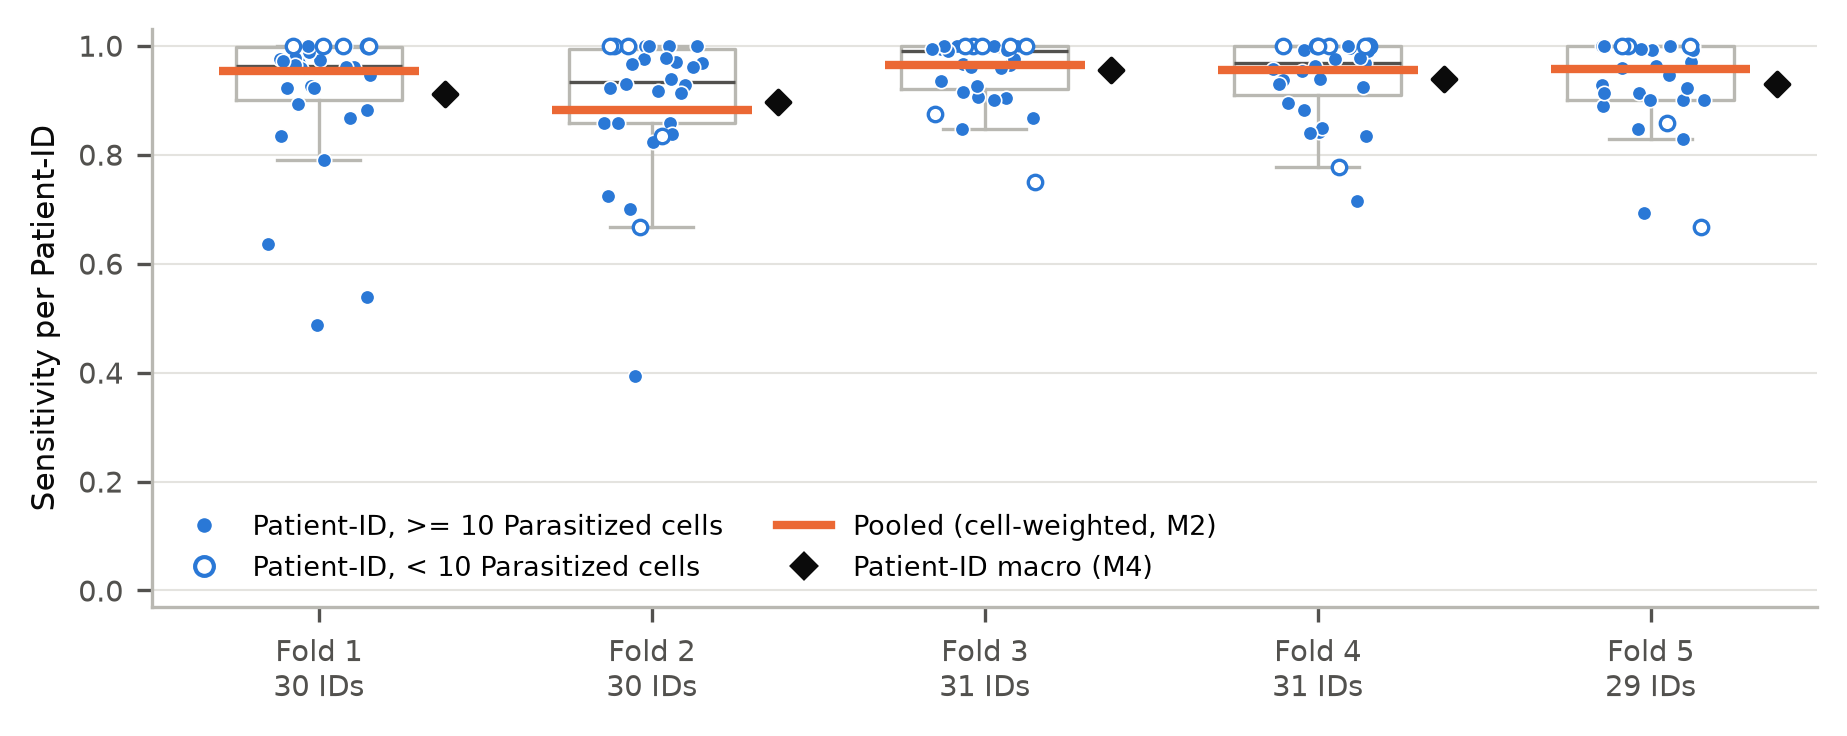
\includegraphics[width=\textwidth]{per_id_sensitivity_by_fold.png}
\caption{Sensitivity of every \pid{} with Parasitized cells, per test fold. Orange bar: pooled (cell-weighted, M2) sensitivity. Black diamond: \pid{}-macro. Hollow markers: \pid{}s with fewer than 10 Parasitized cells.}
\label{fig:perid}
\end{figure*}

\begin{figure*}[t]
\centering
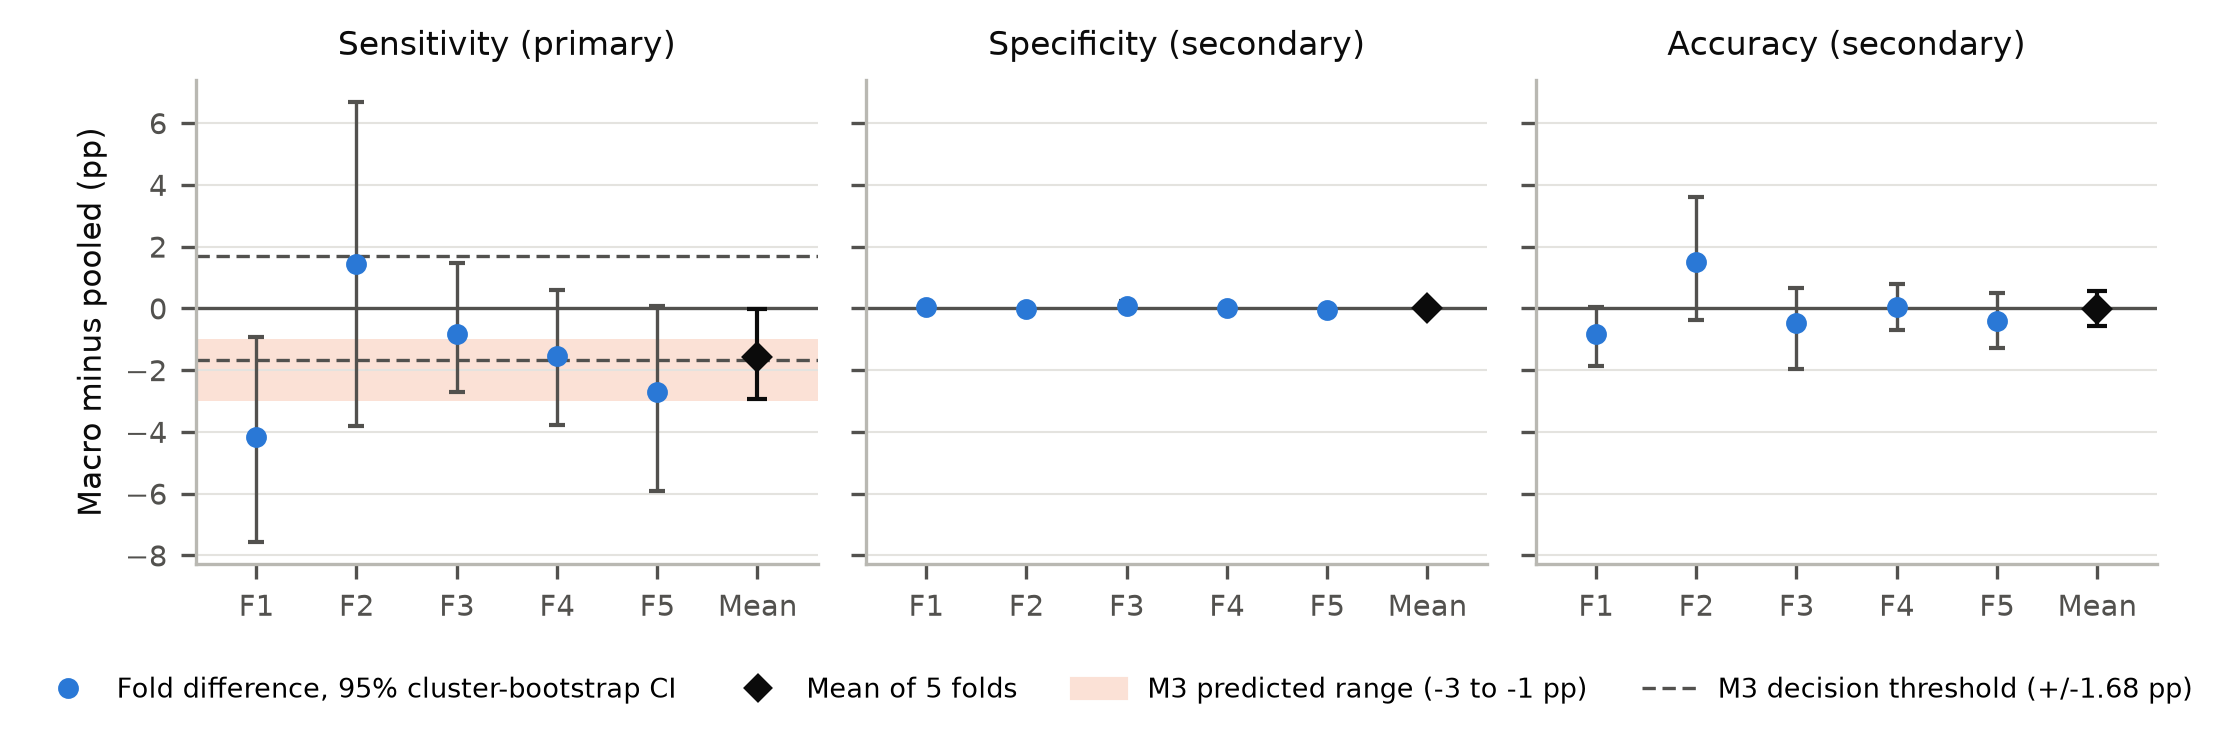
\includegraphics[width=\textwidth]{paired_differences.png}
\caption{Macro minus pooled per fold, with 95\% cluster-bootstrap CIs (A4). The left panel is the pre-registered primary metric: the shaded band is the M3 prediction and the dashed lines are the $\pm1.68$\,pp decision threshold. Specificity and accuracy are secondary.}
\label{fig:diffs}
\end{figure*}

\textbf{Primary result.} Table~\ref{tab:primary} and Fig.~\ref{fig:diffs} give the five paired differences. \val{n_negative_folds} of \val{n_folds} are negative; fold~\val{positive_fold} is positive (\val{positive_fold_diff}). The mean is \val{mean_diff_pp}, \val{within_band} the predicted $-1$ to $-3$\,pp range, but \val{shortfall_pp} short of the $-1.68$\,pp threshold. \emph{Prediction vs.\ outcome:} the direction held in \val{n_negative_folds} folds and the magnitude fell inside the predicted range. The pre-registered threshold was not met, so the verdict is \textbf{\val{verdict}}. Using the threshold's exact source value (\val{threshold_exact_pp}\,pp) gives the same verdict. The 95\% cluster-bootstrap CI for the mean is \val{boot_ci}. It excludes zero and includes $-1.68$\,pp. The across-fold $t$-interval, \val{t_ci}, is wider. Pooled M2 metrics are unchanged by construction.

\begin{table}[t]
\centering
\caption{Primary result: pooled vs.\ \pid{}-macro sensitivity per fold. Verdict under the M3 rule: \val{verdict}.}
\label{tab:primary}
\footnotesize
\setlength{\tabcolsep}{2.5pt}
\resizebox{\columnwidth}{!}{% Generated by paper/make_tables.py from results/. Do not edit by hand.
\begin{tabular}{lrrrrr}
\toprule
\textbf{Fold} & \textbf{IDs} & \textbf{Pooled (\%)} & \textbf{Macro (\%)} & \textbf{$\Delta$ (pp)} & \textbf{95\% CI (pp)} \\
\midrule
1 & 30 & 95.31 & 91.15 & $-$4.16 & [$-$7.58, $-$0.93] \\
2 & 30 & 88.28 & 89.72 & +1.45 & [$-$3.81, 6.68] \\
3 & 31 & 96.38 & 95.55 & $-$0.83 & [$-$2.72, 1.48] \\
4 & 31 & 95.52 & 93.97 & $-$1.55 & [$-$3.79, 0.58] \\
5 & 29 & 95.71 & 92.99 & $-$2.72 & [$-$5.91, 0.08] \\
Mean & 151 & 94.24 & 92.68 & $-$1.56 & [$-$2.95, $-$0.04] \\
\bottomrule
\end{tabular}
}
\end{table}

\textbf{Secondary metrics.} Per-\pid{} sensitivity varies more than per-\pid{} accuracy in \val{folds_sens_sd_gt_acc_sd} of 5 folds: the SD across folds is \val{id_sens_sd_min}--\val{id_sens_sd_max} for sensitivity vs.\ \val{id_acc_sd_min}--\val{id_acc_sd_max} for accuracy (Fig.~\ref{fig:perid}). Macro and pooled specificity almost coincide (mean \val{a5_spec_mean}, CI \val{a5_spec_ci}). The reason is structural: every \pid{} contributes \val{nneg_min}--\val{nneg_max} Uninfected cells, but between \val{npos_min} and \val{npos_max} Parasitized cells (median \val{npos_median}). Accuracy moves by \val{a5_acc_mean} (CI \val{a5_acc_ci}).

\textbf{Ablations (exploratory).} Table~\ref{tab:ablations} summarises them. A1 confirms that cell-count weighting of per-\pid{} sensitivity reproduces the pooled value exactly, in every fold. With A2's $k\ge10$ eligibility, the mean becomes \val{a2_k10_mean}, which would pass the threshold; with $k\ge25$ it becomes \val{a2_k25_mean}, which would not. Neither replaces the pre-registered $k\ge1$ rule. Under A3, single-\pid{} deletions keep the mean between \val{a3_mean_min} and \val{a3_mean_max}. \val{a3_flips} of them flip the verdict: \val{a3_flip_ids}. The most influential is \val{a3_top_id}, with \val{a3_top_npos} Parasitized cells at sensitivity \val{a3_top_sens}. Removing it alone turns fold~\val{a3_top_fold}'s difference to \val{a3_top_diff_without}.

\begin{table*}[t]
\centering
\caption{Exploratory ablations: aggregation only, model untouched. They do not change the primary verdict.}
\label{tab:ablations}
\footnotesize
\resizebox{\textwidth}{!}{% Generated by paper/make_tables.py from results/. Do not edit by hand.
\begin{tabular}{lllrrl}
\toprule
\textbf{Ablation (exploratory)} & \textbf{Setting} & \textbf{IDs} & \textbf{Mean $\Delta$ (pp)} & \textbf{Folds $<$ 0} & \textbf{Note} \\
\midrule
Primary (M3 rule) & macro, $\geq$ 1 Parasitized cell & 151 & $-$1.56 & 4/5 & verdict INCONCLUSIVE \\
A1 weighting & per-ID, weighted by cells & 151 & -- & - & identical to pooled in all folds (max abs. difference 0.0e+00) \\
A2 eligibility & $\geq$ 10 Parasitized cells & 121 & $-$2.00 & 4/5 & 98.9\% of positive cells kept \\
A2 eligibility & $\geq$ 25 Parasitized cells & 84 & $-$1.28 & 4/5 & 94.5\% of positive cells kept \\
A3 leave-one-ID-out & 151 single-ID deletions & 150 remain & -- & - & mean range $-$2.00 to $-$1.27; 2 change the verdict \\
A4 cluster bootstrap & 2,000 resamples, seed 42 & 151 & $-$1.56 & - & 95\% CI [$-$2.95, $-$0.04] \\
A5 specificity & macro over IDs with Uninfected cells & 201 & +0.01 & 3/5 & 95\% CI [$-$0.03, 0.05] \\
A5 accuracy & macro over all IDs & 201 & $-$0.03 & 3/5 & 95\% CI [$-$0.57, 0.55] \\
\bottomrule
\end{tabular}
}
\end{table*}

\section{Failure Analysis}
\textbf{Where the errors are.} The \val{fn_total} false negatives occur in \val{fn_ids_any} of \val{fn_ids_at_risk} eligible \pid{}s. The top \pid{} (\val{fn_top1_id}) holds \val{fn_top1_share}, the top ten hold \val{fn_top10_share}, and \val{fn_ids_50} \pid{}s account for half (Fig.~\ref{fig:conc}). False positives are more diffuse: the top ten hold \val{fp_top10_share}, and \val{fp_ids_50} \pid{}s are needed for half. \pid{}s with at least 100 Parasitized cells contribute \val{fn_share_big_ids} of false negatives. Fold~\val{positive_fold} has the most false negatives (\val{posfold_fn}) and contains \val{fn_top10_in_posfold} of the ten worst \pid{}s. Its top \pid{} alone holds \val{posfold_top_fn_share} of the fold's false negatives. This explains the one positive fold. When large \pid{}s are \emph{hard}, cell weighting pulls pooled sensitivity below the macro, so the hypothesised masking runs in reverse. In the largest-SD fold (fold~\val{sd_fold}), no single \pid{} drives the spread: removing the most influential one, \val{sd_driver}, cuts the SD by \val{sd_reduction_share}.

\begin{figure}[t]
\centering
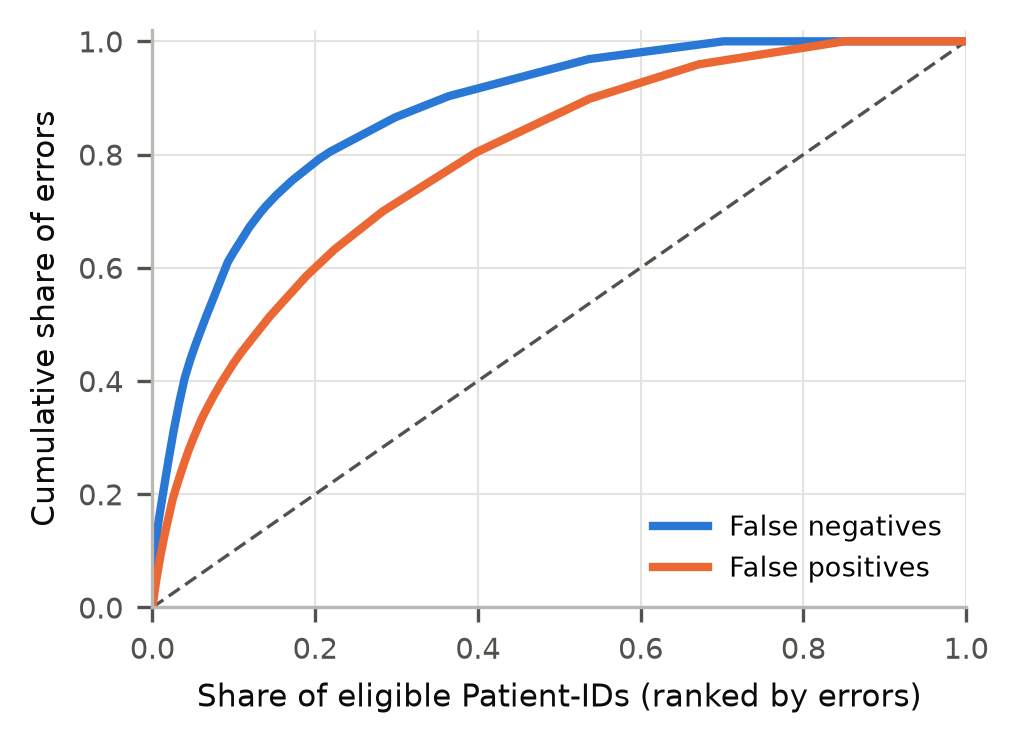
\includegraphics[width=0.92\columnwidth]{error_concentration.png}
\caption{Cumulative share of errors held by \pid{}s ranked from most to fewest errors. Dashed: equal share.}
\label{fig:conc}
\end{figure}

\textbf{Confidence and calibration.} \val{conf_fn} false negatives have $p<0.1$ (\val{conf_fn_share} of all false negatives), and \val{conf_fp} false positives have $p>0.9$ (\val{conf_fp_share}). The Brier score is \val{brier} and the ECE \val{ece} (Fig.~\ref{fig:rel}). Fold~\val{brier_worst_fold} is worst, with a Brier score of \val{brier_worst}. Mid-range bins over-estimate the Parasitized probability by up to \val{cal_max_gap}.

\begin{figure}[t]
\centering
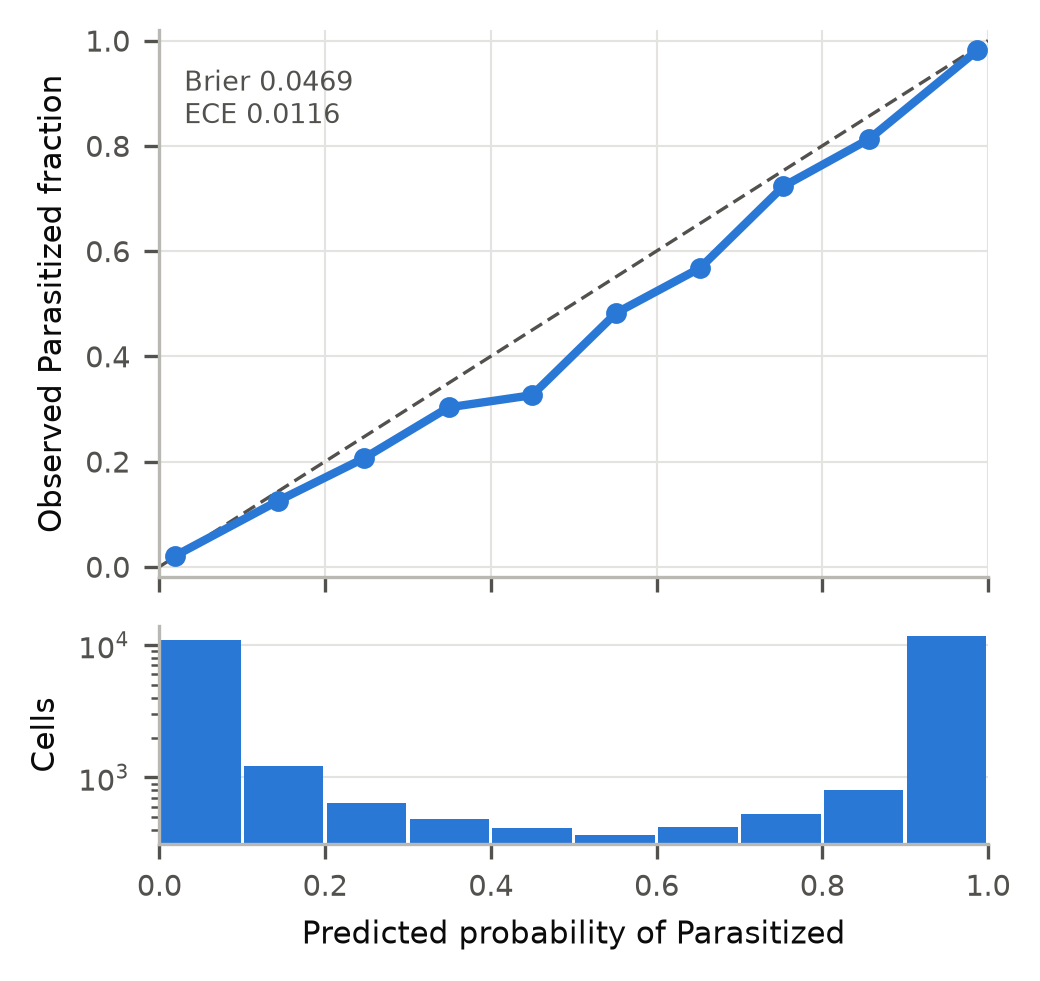
\includegraphics[width=0.85\columnwidth]{reliability_diagram.png}
\caption{Reliability diagram of the out-of-fold probabilities (10 equal-width bins) with bin counts (log scale).}
\label{fig:rel}
\end{figure}

\textbf{Image review.} One reviewer labelled \val{rev_total} crops blind to class, probability and \pid{}: 24 lowest-$p$ false negatives, 24 highest-$p$ false positives, and 24 random true positives and true negatives. The reviewer was the AI assistant used for the analysis, \emph{not} a microscopist, and the categories were fixed before viewing (Table~\ref{tab:review}, Fig.~\ref{fig:grids}). Among random correct cells, a stained inclusion was seen in \val{rev_rtp_inclusion_yes}/24 true positives and \val{rev_rtn_inclusion_yes}/24 true negatives. Among the most confident false negatives, \val{rev_tfn_inclusion_no}/24 showed \emph{no} visible inclusion; among the most confident false positives, \val{rev_tfp_inclusion_yes}/24 showed one. Grey/blue-tinged crops were more frequent among confident false negatives (\val{rev_tfn_pale_or_atypical_stain}/24) than among random true positives (\val{rev_rtp_pale_or_atypical_stain}/24). These are \emph{observations, not causes}. They are consistent with label noise in the segmented crops~\cite{wilm2025coco}, but equally with faint parasites, debris at the crop border, or reviewer error.

\begin{table*}[t]
\centering
\caption{Blind image review: counts per group (one non-expert reviewer, categories fixed in advance). ``Possible label noise'' is derived by code: the visible content disagrees with the dataset label.}
\label{tab:review}
\footnotesize
\resizebox{\textwidth}{!}{% Generated by paper/make_tables.py from results/. Do not edit by hand.
\begin{tabular}{lrrrrrrrrr}
\toprule
\textbf{Group (blind review)} & \textbf{Cells} & \textbf{IDs} & \textbf{Inclusion yes} & \textbf{No} & \textbf{Unclear} & \textbf{Grey/blue or atypical stain} & \textbf{Blur} & \textbf{Segmentation artefact} & \textbf{Possible label noise} \\
\midrule
Top FN (lowest p) & 24 & 17 & 2 & 17 & 5 & 20 & 0 & 4 & 17 \\
Top FP (highest p) & 24 & 22 & 21 & 0 & 3 & 8 & 0 & 8 & 21 \\
Random TP & 24 & 19 & 24 & 0 & 0 & 9 & 1 & 8 & 0 \\
Random TN & 24 & 24 & 0 & 21 & 3 & 13 & 0 & 4 & 0 \\
\bottomrule
\end{tabular}
}
\end{table*}

\begin{figure*}[t]
\centering
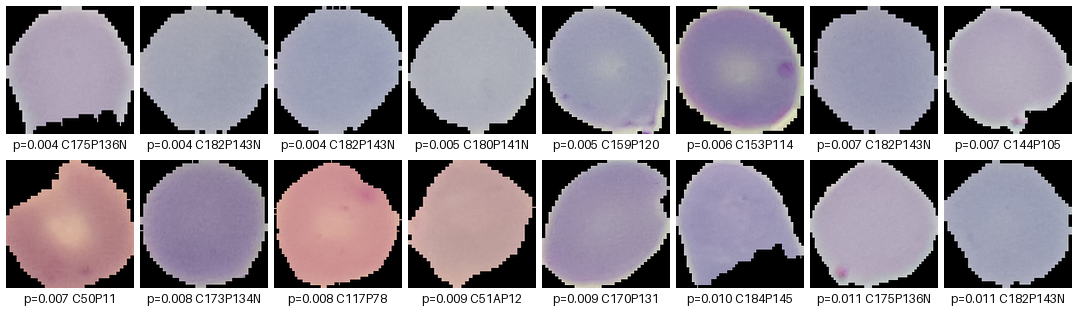
\includegraphics[width=0.93\textwidth]{grid_top_false_negatives.png}\\[2pt]
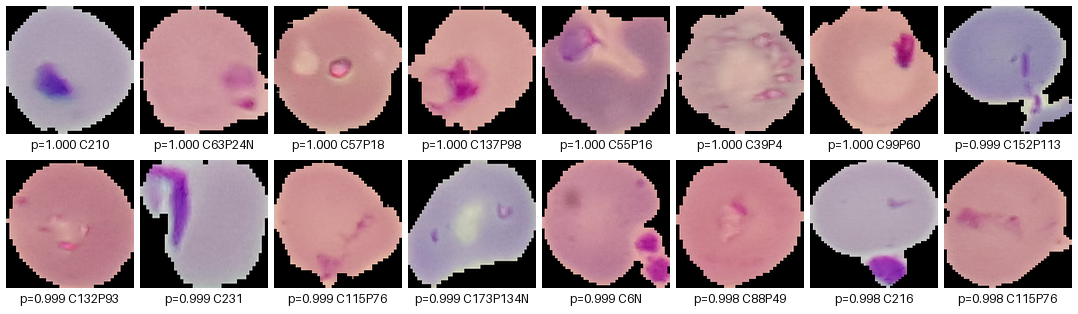
\includegraphics[width=0.93\textwidth]{grid_top_false_positives.png}
\caption{Top: the 16 most confident false negatives (labelled Parasitized, lowest $p$). Bottom: the 16 most confident false positives (labelled Uninfected, highest $p$). Captions: $p$ = P(Parasitized) and the \pid{} prefix (display only). Crops are resized; colours are unaltered.}
\label{fig:grids}
\end{figure*}

\section{Discussion}
The prediction was half right. Cell weighting does mask hard \pid{}s in most folds, and the average effect is about the predicted size. Its direction, however, depends on whether a fold's large \pid{}s happen to be easy or hard. With \val{pos_ids_per_fold} eligible \pid{}s in the five folds and Parasitized counts spanning two orders of magnitude, a few large \pid{}s decide the sign. That is why one fold reverses and why single deletions flip the verdict. The practical lesson for reporting is that pooled and macro sensitivity answer different questions. A pooled value describes cells; a macro value describes the typical source group. Reporting both, with the per-group distribution and the count of groups with undefined sensitivity, shows variation that a single pooled number hides, such as a per-\pid{} sensitivity of \val{id_sens_min} (\val{id_sens_min_id}, \val{id_sens_min_npos} Parasitized cells) in Fig.~\ref{fig:perid}. The failure analysis suggests that some of the hardest ``errors'' may be label questions rather than model questions. Testing that would need expert re-annotation, which is outside this one-change study.

\section{Limitations}
\begin{itemize}
\item \textbf{Five folds, one fold assignment.} All paired statements rest on $n=5$, so no significance can be claimed. Another grouping seed would regroup \pid{}s and could change individual fold signs.
\item \textbf{Fragile verdict.} The outcome is near the threshold: an eligibility change (A2) or a single deletion (A3) moves it. We report the pre-registered verdict and do not adopt the more favourable exploratory variants.
\item \textbf{The \pid{} is a mapping key, not a slide.} Uninfected crops include cells from infected slides, and one source patient has two microscope-specific keys. Results do not transfer to slide-level or patient-level diagnosis.
\item \textbf{Approximate reproduction.} Folds, feature layer, normalisation and classifier differ from~\cite{rajaraman2018}, and specificity is lower than published. The failure modes describe this model.
\item \textbf{Image review.} One non-expert reviewer on \val{rev_total} small crops, with no inter-rater agreement. The top-error groups were selected by model confidence.
\item \textbf{Scope.} One public dataset of segmented \emph{P.~falciparum} thin-smear cells, with no external data. This is not a clinical or diagnostic claim.
\end{itemize}

\section{Conclusion}
We reproduced a patient-level ResNet-50 malaria cell baseline approximately and pre-registered a single evaluation change. Patient-ID--macro sensitivity was lower than pooled sensitivity in \val{n_negative_folds} of \val{n_folds} folds by \val{mean_diff_pp} on average. That falls inside the predicted range but not past the pre-registered threshold, so the verdict is \val{verdict}. The fold that reversed, and the fragility of the verdict, both follow from a few large \pid{}s. Reporting pooled and per-group sensitivity side by side, with the group distribution, is a cheap way to make that structure visible. Next steps, each a separate intervention, are repeated grouping seeds, expert review of the confident errors, and stain-aware analysis.

\bibliographystyle{IEEEtran}
\bibliography{references}

\end{document}
